%%%%%%%%%%%%%%%%%%%%%%%%%%%%%%%%%%%%%%%%%%%%%%%%%%%%%%%%%%%%%%%%
%%%%%%%%%%%%%%%%%%%%%%%%%%%%%%%%%%%%%%%%%%%%%%%%%%%%%%%%%%%%%%%%
%%%%%%%%%%%%%%%%%%%%%%%%%%%%%%%%%%%%%%%%%%%%%%%%%%%%%%%%%%%%%%%%
\eglabel{6}
\section{Example \theexamples: Estimation with IOV}
\label{sec:eg6}

%%%%%%%%%%%%%%%%%%%%%%%%%%%%%%%%%%%%%%%%%%%%%%%%%%%%%%%%%%%%%%%%
\subsection{Description}

In this example we will look at more complex trial design and a
correspondingly complex variability model. The model also includes
categorical covariates, which is again something we have not
encountered thus far. The example is based on example IOV1 from
Monolix 4.1 (see \cite{Monolix4.1.4UserGuide:2012} for a detailed
description) and features a cross-over design and inter-occasion
variability (see section \ref{sec:variabilityModel}). As before we will
go through the key elements of the model before we look at the
\pharmml examples, but given the complex nature of the trial design we
will describe that first then move onto the model definition.


\begin{figure}[htb]
\centering
 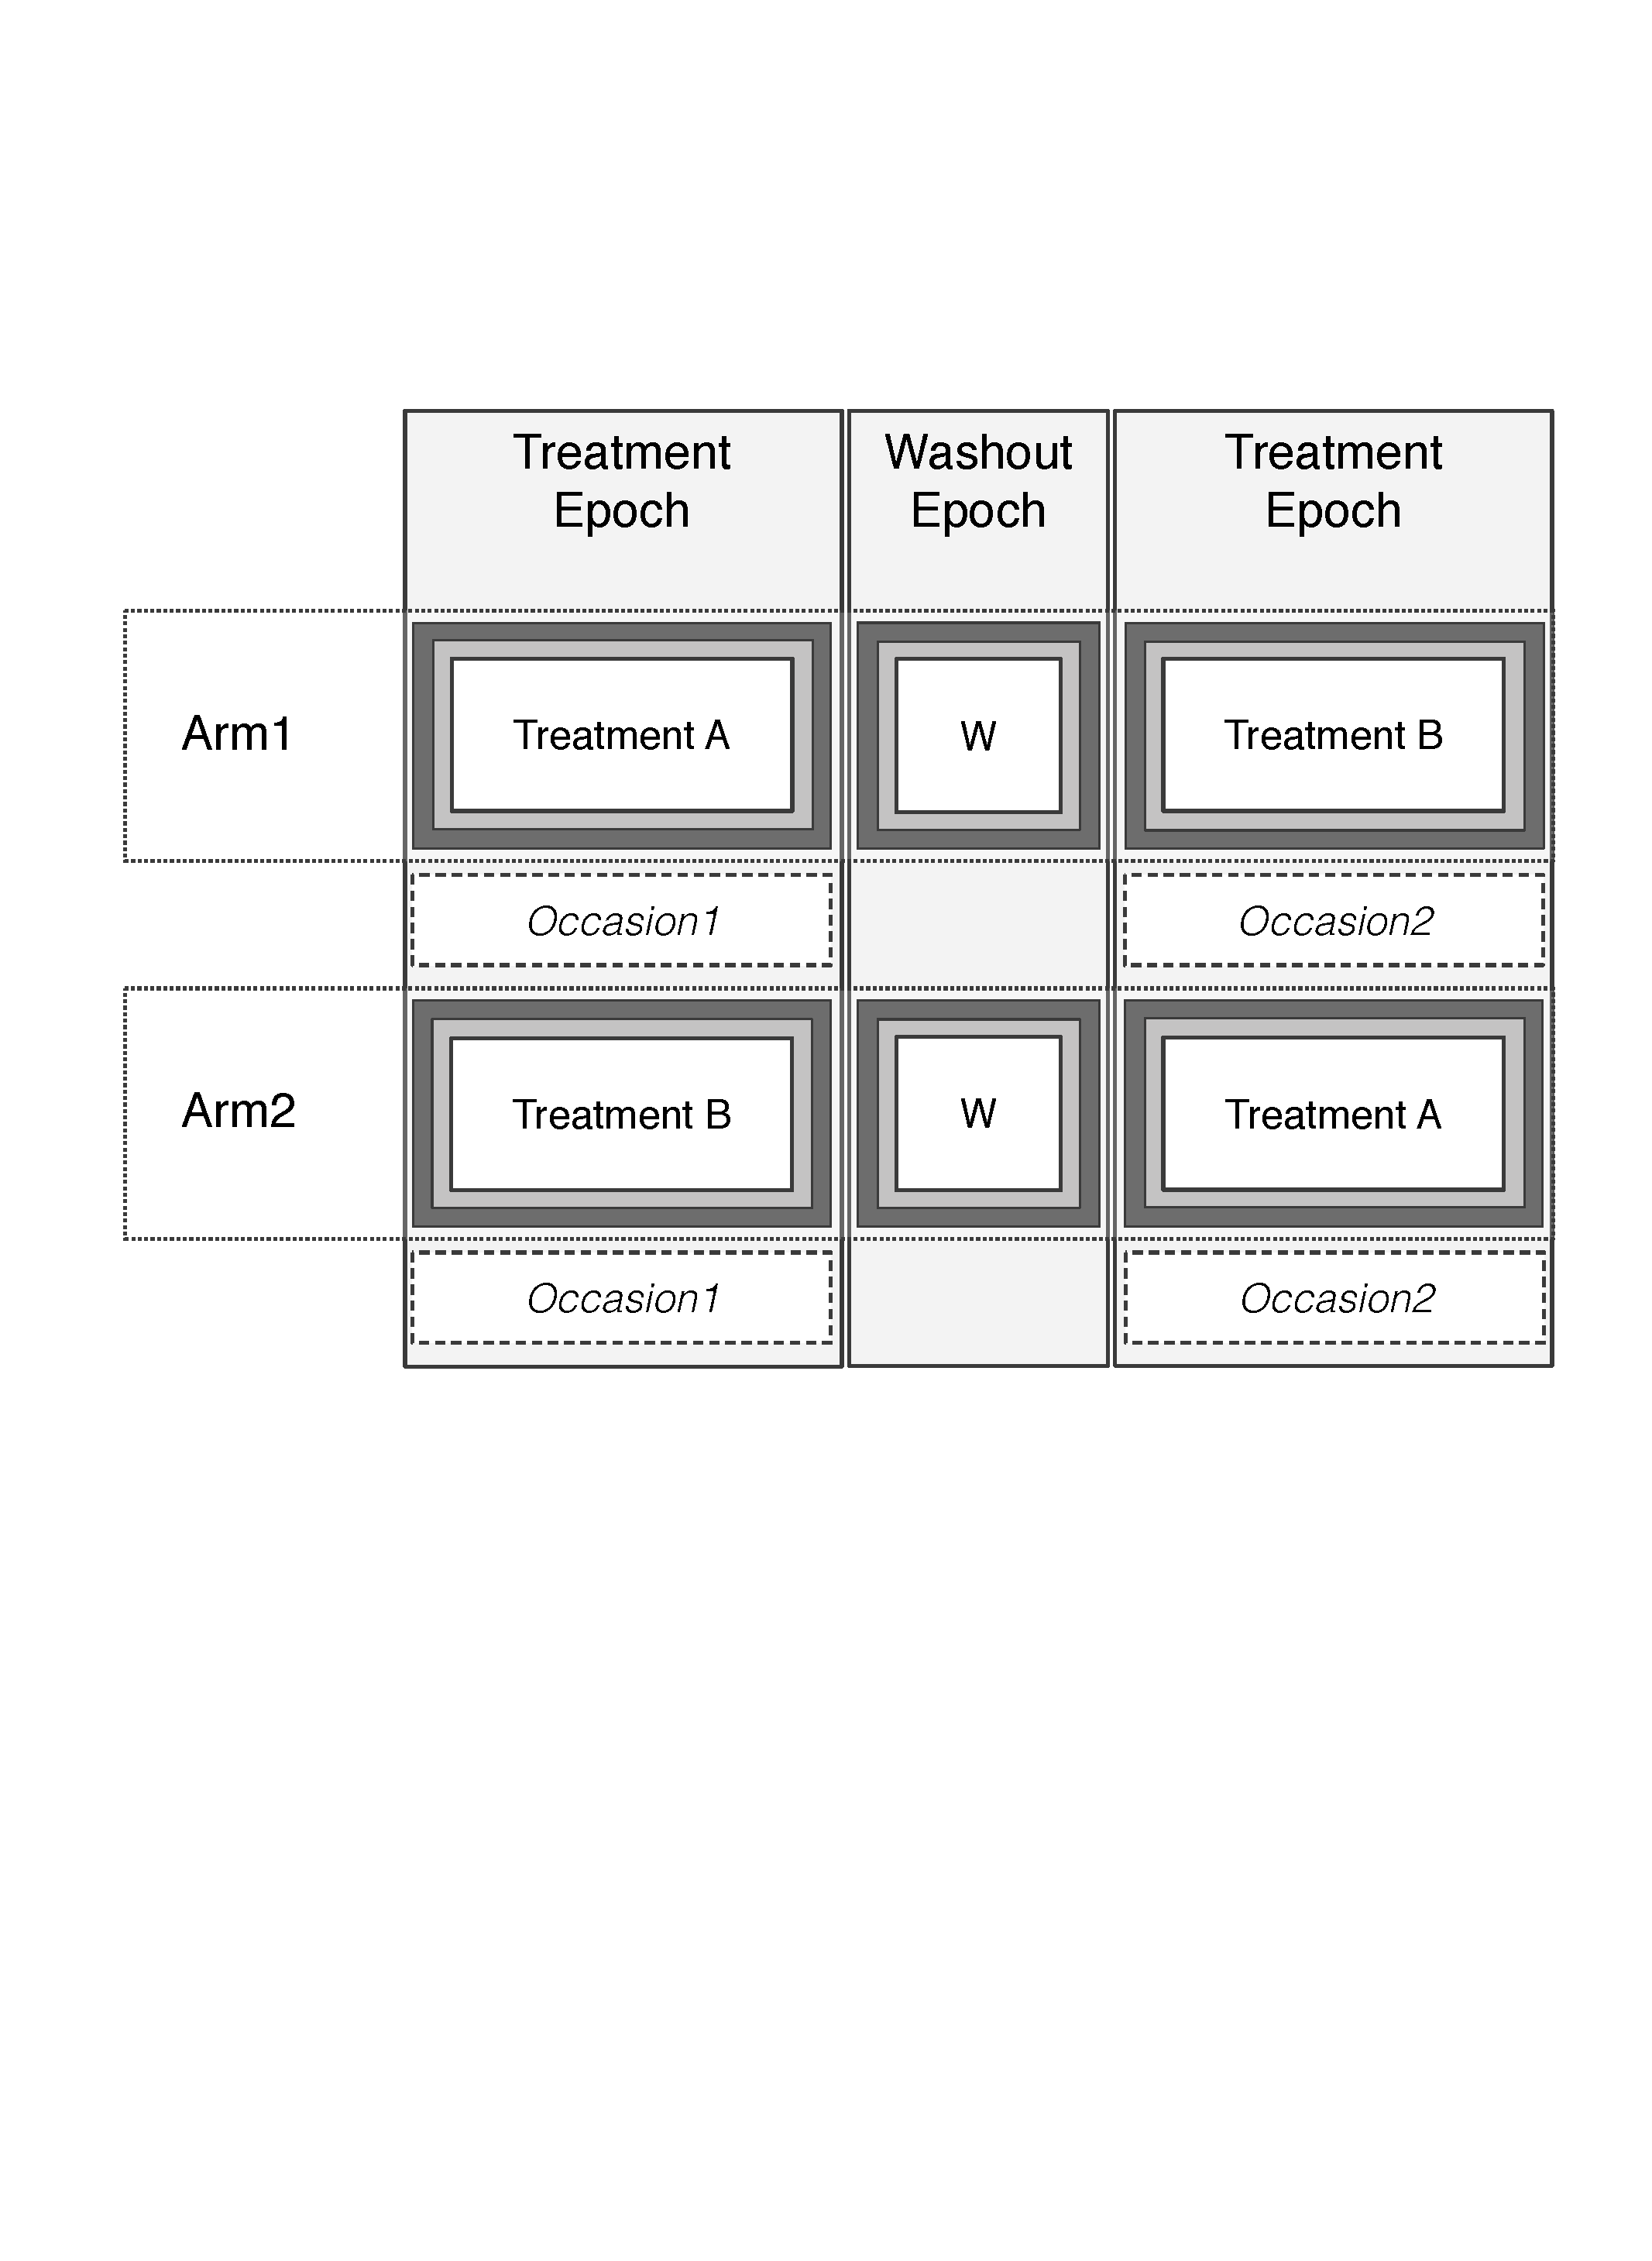
\includegraphics[width=0.7\linewidth]{TwoArmsThreeEpochs_withWashout.pdf}
\caption{Schematic representation of a crossover design with washout. The reader is referred to
Figure \ref{fig:templateTrialDesign} for the colour code used to identify the elements of
a trial. See tables \ref{fig:eg6:segmentCellArmEpoch} 
and \ref{fig:eg6:epochDef} for the detailed definition of segments, cells, arms, epochs
and occasions in this example.}
\label{fig:TwoArmsThreeEpochs_withWashout}
\end{figure}

%\noindent
\begin{table}[h]
\begin{center}
\begin{tabular}{lrr}\toprule
Arm & \textbf{1} & \textbf{2} \\\midrule
Number of subjects & 33 & 33\\
Dose variable & \var{D} & \var{D} \\
Dosing Amount & 100 & 150 \\
Dose Units & $\mg$ & $\mg$  \\
Dose per kg & no & no \\
Dosing times (h) &  [0 : 12 : 72] &  [0 : 12 : 72\\
\bottomrule
\end{tabular}
\end{center}
\caption{Arms overview with dosing specification.}
\label{tab:ArmOverview}
\end{table}


%%%%%%%%%%%%%%%%%%%%%%%%%%%%%%%%%%%%%%%%%%%%%%%%%%%%%%%%%%%%%%%%
\subsubsection{Trial Design}
The model features a basic crossover design (see Figure
\ref{fig:TwoArmsThreeEpochs_withWashout}) with washout period and inter-occasion
variability (IOV). There are two treatments and the subjects are
organised into two arms that start with a different treatment. In
between each treatment there is a washout period during which time the
drug is eliminated from each subject. 
In the model the treatments, fi treated as occasions, provide a second level of variability -- 
IOV \index{variability!IOV} (see section \ref{sec:variabilityModel}).  
This is summarised in Figure \ref{fig:eg6-IOV_2levels} (see also the listing 
in section \ref{eg6:variabilityModel}, showing relevant code 
within the element \xelem{VariabilityModel}).

The model also uses covariates to model the variability within the
model and so the treatments, the sequence of treatments (i.e.\xspace treatments A, B or
B,A) and the occasion itself are described in the covariate section
below.

\begin{figure}[ht!]
\centering
 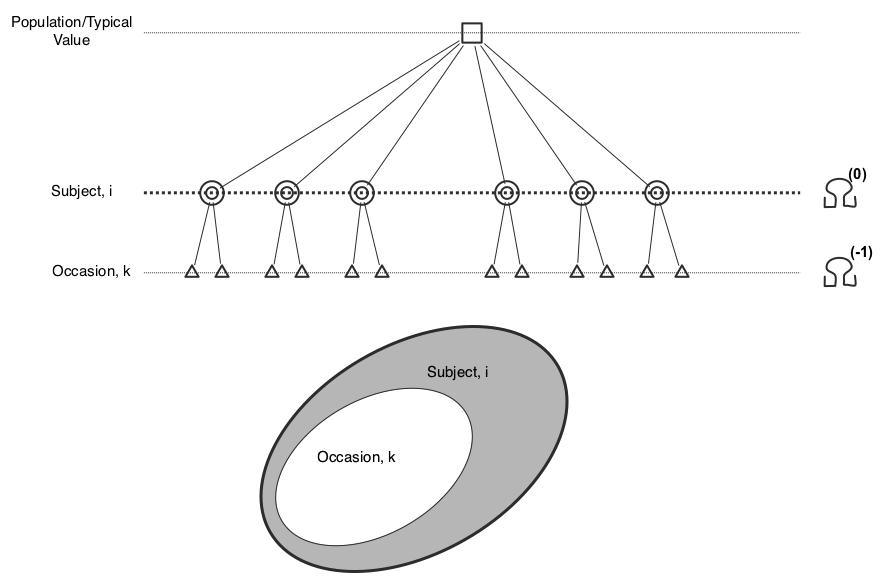
\includegraphics[width=120mm]{IOV_2levels}
\caption{Two levels of variability -- inter-individual and inter-occasion within individual variability.}
\label{fig:eg6-IOV_2levels}
\end{figure}


%%%%%%%%%%%%%%%%%%%%%%%%%%%%%%%%%%%%%%%%%%%%%%%%%%%%%%%%%%%%%%%%
\subsubsection{Covariate Model}
\label{eg6:covariates-defn}

As discussed about all but the `Sex' covariate is used to capture the
variability in the model, see Table \ref{tab:CovariatesOverview}.

\begin{table}[h]
\begin{center}
\begin{tabular}{lrrrr}\toprule
 & \textbf{Sex} &{\color{red}\textbf{Treat}}&{\color{mediumgreen}\textbf{TreatSeq}}&{\color{magenta}\textbf{Occasion}}\\\midrule
Type & Categorical & Categorical & Categorical & Categorical  \\
Category Count & 2 & 2 & 2 & 2\\
Categories & F, M & A, B & A--B,B--A & 1, 2\\
Reference & F & A & A--B & 1\\
%Reference Probability & $14/36$ & 0.5  & 0.5  & 0.5\\
\bottomrule
\end{tabular}
\end{center}
\caption{Covariates overview.}
\label{tab:CovariatesOverview}
\end{table}

%%%%%%%%%%%%%%%%%%%%%%%%%%%%%%%%%%%%%%%%%%%%%%%%%%%%%%%%%%%%%%%%
\subsubsection{Parameter Model}

The parameter model includes random effects that represent the IIV and
{\color{lightblue}IOV} levels of variability. It also relates the
parameters to the covariates described above\footnote{To improve
  clarity we have colour coded the contributions of the different levels
of variability and the different covariates.}

\begin{align}
\log(ka_{i}) &= \log(ka_{pop}) +
{\color{mediumgreen}\beta_{ka,TreatSeq}}1_{TreatSeq_i=A-B} +
\eta_{ka,i} \label{eqn:eg6-param-ka}\\
\begin{split}
\log(V_{ik}) &= \log(V_{pop}) + {\boldsymbol \beta_V}1_{S_i=F} +
{\color{magenta}\beta_{V,OCC}} 1_{OCC_{ik}=1} \\
&\quad+ {\color{red}\beta_{V,Treat}}1_{Treat_{ik}=A} + {\color{mediumgreen}\beta_{V,TreatSeq}}1_{TreatSeq_i=A-B} \\
		& \quad+ \eta_{V,i}^{(0)} +  {\color{lightblue} \eta_{V,ik}^{(-1)} }
\end{split} \label{eqn:eg6-parameter-v}\\
\begin{split}
\log(\CL_{ik}) &= \log(\CL_{pop}) + {\boldsymbol \beta_{\CL}}1_{S_i=F}
+ {\color{magenta}\beta_{\CL,OCC}} 1_{OCC_{ik}=1}\\
&\quad + \eta_{\CL,i}^{(0)} + {\color{lightblue} \eta_{Cl,ik}^{(-1)} }
\end{split}\nonumber
\end{align}
where
\begin{gather*}
\eta_{ka,i}^{(0)} \sim \mathcal{N}(0, \omega_{ka}), \quad \eta_{V,i}^{(0)} \sim \mathcal{N}(0, \omega_{V}), \quad \eta_{\CL,i}^{(0)} \sim \mathcal{N}(0, \omega_{\CL}),  \\
 {\color{lightblue} \eta_{V,ik}^{(-1)} \sim \mathcal{N}(0,\gamma_V)}, \quad
 {\color{lightblue} \eta_{\CL,ik}^{(-1)} \sim \mathcal{N}(0, \gamma_{\CL})}
\end{gather*}

The full variance-covariance matrix for our model is :
\begin{gather}
 \Omega^{(0)} =
 \begin{pmatrix}
  \omega_{ka}^2 	& 0 				& 0  \\
   			  	& \omega_{V}^2	& 0 	\\
  				& 				& \omega_{\CL}^2\\
 \end{pmatrix}\label{eqn:eg6-covariance-mat}\\
 \Omega^{(-1)} =
 \begin{pmatrix}
0 & 0 & 0\\
 & \gamma_{V}^2	& 0 	\\
 & & \gamma_{\CL}^2\\
 \end{pmatrix}\label{eqn:eg6-gamma-mat}
\end{gather}


%%%%%%%%%%%%%%%%%%%%%%%%%%%%%%%%%%%%%%%%%%%%%%%%%%%%%%%%%%%%%%%%
\subsubsection{Structural model}

The model is first order absorption with linear elimination, with
multiple dosing. This is the equivalent to oral1\_1cpt\_kaVCl (model 8) from \cite[Appendix I]{Bertrand:2008}.


%%%%%%%%%%%%%%%%%%%%%%%%%%%%%%%%%%%%%%%%%%%%%%%%%%%%%%%%%%%%%%%%
\subsubsection{Observation model}

We apply a residual error models to the output variable \var{C}.

%\noindent
\begin{center}
\begin{tabular*}{0.6\textwidth}{@{\extracolsep{\fill}} >{\bfseries}l l}\toprule
Output Variable  & \textbf{\itshape C} \\\midrule
Observations Name & Concentration\\
Units & $\mg/l$ \\
Observations Type & Continuous \\
Residual Error Model & Combined \\
Error Model Parameters & $a = 0.1,\quad b=0.1$\\
\bottomrule
\end{tabular*}
\end{center}


%%%%%%%%%%%%%%%%%%%%%%%%%%%%%%%%%%%%%%%%%%%%%%%%%%%%%%%%%%%%%%%%
\subsubsection{Modelling Steps}
Compared to the last example, we have define here two tasks:
\begin{itemize}
\item Estimation of population paramaters.
\item Estimation of the individual parameters.
\end{itemize}

%%%%%%%%%%%%%%%%%%%%%%%%%%%%%%%%%%%%%%%%%%%%%%%%%%%%%%%%%%%%%%%%
\subsection{Trial Design}

We have summaries the dosing regimen and organisation of the trial
design below, see also Figure \ref{fig:TwoArmsThreeEpochs_withWashout}.

\begin{table}[htdp!]
\begin{center}
\begin{tabular}{ccccccc}
\hline
Segment&Activity & Treatment & DoseTime & DoseSize & Target Variable \\
\hline
TA& OR1 &  OR bolus & $0:12:72$ & 150 & Ac \\
TA& OR2 &  OR bolus & $0:24:72$ & 100 & Ac \\
\hline
\end{tabular}
\end{center}
\caption{Segment/activity overview.}
\label{fig:eg6:segmentCellArmEpoch}
\end{table}

\begin{table}[htdp!]
\begin{center}
\begin{tabular}{cccc}
\hline
Epoch & Occasion & Start time & End time \\
\hline
Treatment Epoch & OCC1 & 0 &  180  \\
Washout & -- & 0 &  10  \\
Treatment Epoch & OCC2 & 0 &  180  \\
\hline
\end{tabular}
\end{center}
\caption{Epoch and occasion definition.}
\label{fig:eg6:epochDef}
\end{table}


%%%%%%%%%%%%%%%%%%%%%%%%%%%%%%%%%%%%%%%%%%%%%%%%%%%%%%%%%%%%%%%%
\subsubsection{Structure}
The implementation of the treatments, in \pharmml we use the
\xelem{Activity} element, is different compared to the previous example. 
See Table \ref{fig:eg6:segmentCellArmEpoch} for the details. The difference
is that now we have one dose administered at multiple dosing time points 
instead of single time point. See the following listing \inputxml{exp6_dosingTimes.xml}
how one can describe it within the \xelem{DosingTimes} element using the \xelem{Sequence}
structure defining the start/end times and step size.

Table \ref{fig:eg6:epochDef} gives an overview of the \var{Epochs} and \var{Occasions} 
in this example. Here, the occasions overlap with the epochs, the start and end times 
are identical, this is not always the case, the occasions can span one or more epochs. 
The \var{Washout} epoch is given here with start/end times as well which is in fact 
a redundant piece of information (but required by construction of an \var{Epoch})
as a \var{Washout} always assumes total reset of all drug amounts. 

%\begin{listing}[ht!]
%\inputxml{exp6_structure_part3.xml}
%\caption{The implementation of the mapping of IOV to the trial design.}
%\label{exp6_structure_part3}
%\end{listing}

As discussed in the section \ref{subsec:TrialStructure}, in \xelem{Structure} block 
we encode the variability which is located below the subject (see the 
hierarchy of the random variability discussed in section \ref{sec:variabilityModel}).
We call it the \textit{inter-occasion variability}, IOV. The following listing 
\inputxml{exp6_structure_part3.xml} shows how this is done. 
In this case the occasions coincide with the epochs 
so we use the \xelem{EpochRef} element. Alternatively, we could use the \xelem{Period}
element to define explicitly the start and end times of the occasions as shown 
in this listing: \inputxml{exp6_structure_part4.xml}
This is of course very useful if the occasions do not
coincide with the epochs, or there are two or more occasions within one epoch.
In this case we set the \var{Start} and \var{End} times to $0$ and $180$, respectively.
These are exactly the same time points as are used in the epoch definition 
(see the first listing in section \ref{eg4_subsec:trialDesign} for how to encode epochs in the 
\xelem{Structure} definition).   

%\begin{listing}[ht!]
%\inputxml{exp6_structure_part4.xml}
%\caption{Alternative implementation of the mapping of IOV to the trial design shown in previous listing.}
%\label{exp6_structure_part4}
%\end{listing}
 

%%%%%%%%%%%%%%%%%%%%%%%%%%%%%%%%%%%%%%%%%%%%%%%%%%%%%%%%%%%%%%%%
\subsubsection{Population}
We pick up where we left off in the \xelem{Structure}, implementing
the hooks to the variability structure. The aspect we have not covered
yet is related to IIV.  The \xelem{Population} element is the place to
define any subject related variability and those levels above
it. The following listing shows how this works \inputxml{exp6_population_part0.xml}
Here we deal only with the IIV so we are done with this aspect.

%\begin{listing}[ht!]
%\inputxml{exp6_population_part0.xml}
%\caption{The implementation of the IIV mapping.}
%\label{exp6_population_part0}
%\end{listing}

The next part of the \xelem{Population} block was discussed previously, 
with one exception. Beside the standard assignment of subjects to an \var{Arm}
and providing information regarding \var{Sex}, we need to encode the information
about \var{Treat}, i.e. treatment type considered here as covariate, which varies
by definition in this cross-over design as the study progress from \var{Epoch1}
to \var{Epoch3}. To encode this we use the \textit{nested table} concept as described 
in section \ref{sec:dataset}. 
Here the child table is defined by using a \xelem{Table} element instead of the 
usual \xelem{Column} element and given the identifier 'treat-tab'. 
Within the nested table definition another set of relevant columns is specified, 
\var{epoch} and \var{treat}. Next these nested tables are populated with 
data as can be seen in the following listing \inputxml{exp6_population_part2.xml}
here for \var{Arm1}.
Listing \inputxml{exp6_population_part2B.xml}
shows one data record for \var{Arm2}.

%\begin{listing}[ht!]
%\inputxml{exp6_population_part2.xml}
%\caption{The implementation of the nested table for time varying covariate, \var{Treat}, for  \var{Arm1}.}
%\label{exp6_population_part2}
%\end{listing}

%\begin{listing}[ht!]
%\inputxml{exp6_population_part2B.xml}
%\caption{The implementation of the nested table for time varying covariate, \var{Treat},  for  \var{Arm2}.}
%\label{exp6_population_part2B}
%\end{listing}


%%%%%%%%%%%%%%%%%%%%%%%%%%%%%%%%%%%%%%%%%%%%%%%%%%%%%%%%%%%%%%%%
\subsection{Variability Model}
\label{eg6:variabilityModel}

In this example the variability model is more complex than before, with IIV\index{variability!IIV} and IOV\index{variability!IOV} levels of variability, see Figure \ref{fig:eg6-IOV_2levels}. As you will see, in \pharmml the complexity comes later -- in the parameter model. At this point in the \pharmml document all we need to do is define the variability levels to be used in the rest of the document. You can see in the following listing \inputxml{exp6_iov.xml}
that this is done simply by listing the variability levels using the \xelem{VariabilityLevel} element. There are three important points to note here:
\begin{enumerate}
\item There is parent-child relationship between the levels of variability. The \var{Subject} level, 
in the \pharmml it is referenced with the attribute \xatt{symbId="indiv"} is higher
in the hierarchy and directly above the \var{Occasion} level, referenced with the 
attribute \xatt{symbId="iov1"} which is exactly what is done
using the \xelem{ParentLevel} in the listing above.
\item The name given to a level, using the \xatt{symbId} attribute, is \textbf{not} significant. We used the names \var{iov1} and \var{indiv} to provide clarity in other parts of the example document.
\item the type of each variability level (e.g.,\xspace between-subject, inter-occasion, between-centre) is not defined here or in the Model Definition as a whole\footnote{N.B.,\xspace The numerical levels described in the variability model (section \ref{sec:variabilityModel}) are not used.}.
\end{enumerate}

So in this example the \pharmml document tells us that there are two variability levels and that the lowest level of variability is called ``\texttt{iov1}''\index{variability!IOV}\@. This may seem odd, but to simulate or estimate the model we do not need to know which level of variability is considered IIV and which IOV.  We only need to know their level relative to each other. Of course it may be desirable to know this when exchanging  a model, and we feel that this information can be provided by annotation of the \pharmml document.


%%%%%%%%%%%%%%%%%%%%%%%%%%%%%%%%%%%%%%%%%%%%%%%%%%%%%%%%%%%%%%%%
\subsection{Covariate Model}

The covariate model describes categorical covariates, listed in Table 
\ref{tab:CovariatesOverview}, \index{covariate!categorical}which we have 
not seen in the previous examples. 

Because this is an estimation example no probabilities are provided and only the 
categories are defined, placed in the \xelem{Categorical} element. 
Then the implementation of each covariate follows the same
schema, which will be explained for the gender covariate \var{Sex}. 
There are obviously two categories the covariate can be associate with \textit{F} or \textit{M},
which are encoded using the \xelem{Category} element followed by an optional
\xelem{Name}. 

See the following listing how this is done 
\inputxml{exp6_covariates.xml}

%%% TODO
%%%In a later simulation example (example \egref{8}, section
%%%\ref{eg8:example8}) you will see how to assign probabilities to categorical covariates.


%%%%%%%%%%%%%%%%%%%%%%%%%%%%%%%%%%%%%%%%%%%%%%%%%%%%%%%%%%%%%%%%
\subsection{Parameter Model}

In example \egref{1} (section \ref{sec:eg1}) we showed you how to define an individual
parameter in \pharmml and relate that to a continuous covariate. Now
in this example we will show how \pharmml can be used to describe
parameters that have multiple levels of variability and are related to
categorical covariates\index{covariate!categorical}.


In the following listing \inputxml{exp6_ka.xml} we show the definition of
parameter \var{ka}, which corresponds to (\ref{eqn:eg6-param-ka}). You
should be familiar with this structure by now, but you should take
note of the \xelem{Category} element within the \xelem{FixedEffect}
element. We use this to tell \pharmml that this fixed effect is related
to the ``\texttt{AB}'' category of the \var{TreatSeq} covariate. This
is equivalent to the expression
$\beta_{ka,TreatSeq}1_{TreatSeq_i=A-B}$ in
(\ref{eqn:eg6-param-ka}). Note that it is possible to do this more
than once, for example if the covariate has more than two categories.


Parameter \var{ka} has only one level of variability, but this 
\inputxml{exp6_V_part1.xml} and this listing \inputxml{exp6_V_part2.xml}
show how we describe parameter
\var{V} with both IIV and IOV levels of variability. Very simply we
add a \xelem{RandomVariable} for each level of variability and use
the \xatt{symbIdRef} attribute in the \xelem{RandomEffects} element 
to map the random effect to the appropriate variability model as defined at 
the beginning of the \xelem{ModelDefinition} element. 
Thus \var{eta\_V} and \var{kappa\_V} correspond to the 
random effects $\eta^{(0)}_{V,i}$ and $\eta^{(-1)}_{V,ik}$ in
(\ref{eqn:eg6-parameter-v}). This parameter is related to all four
covariates, but we only show the \var{Sex} covariate. The others
defined in a very similar manner as all the covariates in this model
contain just 2 categories.

%%% TODO
We will not show parameter \var{Cl} as it does not illustrate any new
concepts, nor are any of the random effects in the model
correlated. This does not mean there is no covariance matrix defined
within the \pharmml document. There is. The matrices in
(\ref{eqn:eg6-covariance-mat}) and (\ref{eqn:eg6-gamma-mat}) are
implicitly defined because all the random effects follow a normal
distribution and we can deduce the diagonal of each matrix at each
level of variability from the definition of each random effect.

\subsection{Covered in previous examples}
The remaining elements of this example to be encoded in \pharmml
are nearly identical to those described before, such as \xelem{EstimationStep}
and \xelem{StepDepend\-encies} within the\\ \xelem{ModellingSteps} block,
and will not be discussed here.



%%%%%%%%%%%%%%%%%%%%%%%%%%%%%%%%%%%%%%%%%%%%%%%%%%%%%%%%%%%%%%%%%
%%%%%%%%%%%%%%%%%%%%%%%%%%%%%%%%%%%%%%%%%%%%%%%%%%%%%%%%%%%%%%%%%
%%%%%%%%%%%%%%%%%%%%%%%%%%%%%%%%%%%%%%%%%%%%%%%%%%%%%%%%%%%%%%%%%
%\eglabel{4}
%\section{Example \theexamples: Simulation with IOV}
%\label{sec:eg4}




%%%%%%%%%%%%%%%%%%%%%%%%%%%%%%%%%%%%%%%%%%%%%%%%%%%%%%%%%%%%%%%%
%%%%%%%%%%%%%%%%%%%%%%%%%%%%%%%%%%%%%%%%%%%%%%%%%%%%%%%%%%%%%%%%
%%%%%%%%%%%%%%%%%%%%%%%%%%%%%%%%%%%%%%%%%%%%%%%%%%%%%%%%%%%%%%%%
\eglabel{5}
\section{Example \theexamples: Estimation with individual dosing}
\label{sec:Ribba}

%%%%%%%%%%%%%%%%%%%%%%%%%%%%%%%%%%%%%%%%%%%%%%%%%%%%%%%%%%%%%%%%
\subsection{Description}
This example is based on \cite{Ribba:2012uq} and deals with a mathematical
model describing the inhibition of the tumour growth of low-grade glioma treated
with chemotherapy. Although previous estimation examples were complex
enough to illustrate most important aspects of the current \pharmml specification we would
like briefly to discuss this example due to its role as a use case. It also illustrates a new feature
of the language, the fact that we can encode patient specific administration scenarios.


%%%%%%%%%%%%%%%%%%%%%%%%%%%%%%%%%%%%%%%%%%%%%%%%%%%%%%%%%%%%%%%%
\subsection{Trial design}
We will start with the definition of \xelem{Structure}, \xelem{Population}. The next language element, \xelem{IndividualDosing}, is, as mentioned above, new but it's easy to understand.

%%%%%%%%%%%%%%%%%%%%%%%%%%%%%%%%%%%%%%%%%%%%%%%%%%%%%%%%%%%%%%%%
\subsubsection{Structure}
Figure \ref{fig:1Arm1Epoch_RibbaDesign} shows the design structure of this example 
consisting of one arm and one epoch, meaning there is one treatment type 'IV' for all patients. 
As explained in section \ref{sec:CTS} the design element \xelem{Cell} comprises the 
essential elements specifying the information about the arm, epoch and segment/activities. 
\xelem{Segment} contains treatment definition, here an IV bolus administration, 
defined in the \xelem{Activity} element. Figure \ref{fig:cellHierarchy_Ribba} shows 
the general relationship of these elements (left) and how it applies to the current example (right).
See the following listing 
\inputxml{Ribba_structure.xml}
%\caption{Defining \textit{Structure} of the example, i.e. \textit{Epoch}, \textit{Arm}, \textit{Cell} and \textit{Segment}. \textit{Segment} contains \textit{Activity} definition, here a bolus administration.}
%\label{lst:Ribba_structure}
%\end{listing}
for the PharmML implementation.

\begin{figure}[ht!]
\centering
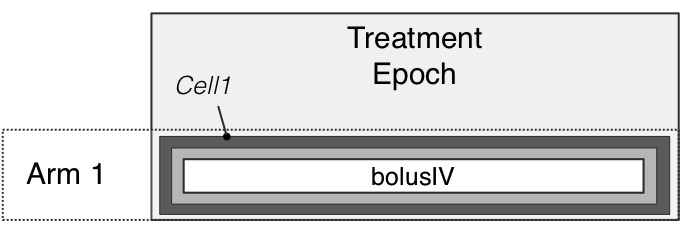
\includegraphics[width=0.7\linewidth]{pics/designPattern_1Arm1Epoch_Ribba}
\caption{Design overview: single arm design.}
\label{fig:1Arm1Epoch_RibbaDesign}
\end{figure}

\begin{figure}[ht!]
\centering
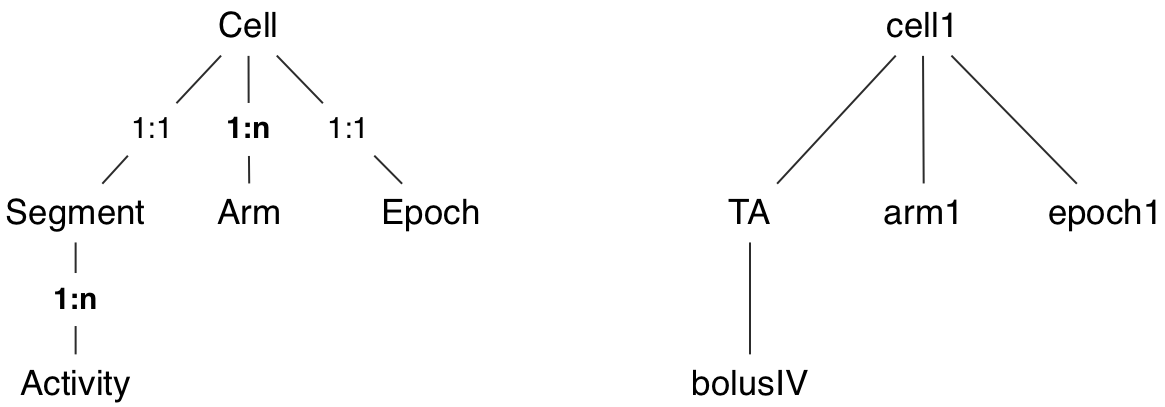
\includegraphics[width=0.7\linewidth]{pics/cellHierarchy_Ribba}
\caption{General cell hierarchy (left); The root of the trial design structure hierarchy is the 'Cell' which can contain one 'Segment',
one 'Epoch' and multiple 'Arms'. The 'Segment' element can have multiple child elements, the 'Activities', e.g. treatments or a washout. (right) An example of how it is applied in \cite{Ribba:2012uq}.}
\label{fig:cellHierarchy_Ribba}
\end{figure}

\begin{table}[htdp!]
\begin{center}
\begin{tabular}{ccccccc}
\hline
Segment&Activity & Treatment & DoseTime & DoseSize & Target Variable \\
\hline
TA& bolusIV &  IV bolus & individual & 1 & C \\
\hline
\end{tabular}
\end{center}
\caption{Segment/activity overview.}
\label{tab:segementActivity_Ribba}
\end{table}

%%%%%%%%%%%%%%%%%%%%%%%%%%%%%%%%%%%%%%%%%%%%%%%%%%%%%%%%%%%%%%%%
\subsubsection{Population}
In the next step, the \textit{Population} is defined, i.e. attributes of the individuals in the study. 
This means creating an individual template with columns for an identifier, arm and repetition and then
populating the table with appropriate data.
As no covariates are used here the \textit{Population} description reduces to the assignment 
of the subjects to the single study arm, \textit{Arm1}. As a shorthand we use the
\textit{repetition} method by defining the column 'rep', as can be seen in the following listing 
\inputxml{Ribba_population.xml}
The identifiers, ID, created here are unique and will be used to the refer to specific subjects 
in the subsequent \xelem{IndividualDosing} structure element described in the following section.


%%%%%%%%%%%%%%%%%%%%%%%%%%%%%%%%%%%%%%%%%%%%%%%%%%%%%%%%%%%%%%%%
\subsubsection{Individual Dosing}
\label{subsubsec:Ribba_indivDosing}

This model utilises the idea of the so called K-PK model, meaning that the rate of the drug entry is relevant
but not its absolute value. Such models often assume, as it is the case here, that the dose is equal 1
for all subject and dosing events, see Table \ref{tab:Ribba_dataSet}.

\begin{table}[htdp]
\begin{center}
\begin{tabular}{rrrr | rrrr | rrrr}\toprule
ID&TIME&DV&DOSE & ID&TIME&DV&DOSE& 			ID&TIME&DV&DOSE \\\midrule
1&0&.&.& 		 	1&116.23&72.04&.& 				20&13.4&.&1\\
1&3.43&45.7&.& 	1&121.87&90.16&.& 				20&17.13&42.62&.\\
1&5.3&48.03&.& 	$\dots$ &$\dots$ &$\dots$ & $\dots$&	21&0&.&.\\
1&42.13&71.34&.& 	$\dots$ &$\dots$ &$\dots$ & $\dots$&	21&1.5&.&1\\
1&52.63&79.3&.& 	20&0&48.61&.&					21&3.17&.&1\\
1&54.57&.&1 & 	20&4&.&1&						21&4.85&.&1\\
1&57.53&72.3&.& 	20&5.88&.&1&						21&6.52&.&1\\
1&59.77&.&1 & 	20&6.7&46.64&.&					21&8.19&.&1\\
1&63.3&72.07&.& 	20&7.76&.&1&						21&9.77&72.35&.\\
1&68.97&70.24&.& 	20&9.27&44.97&.&					21&9.87&.&1\\
1&76.53&66.81&.& 	20&9.64&.&1&						21&14.23&66.96&.\\
1&94.53&60.48&.&	20&11.52&.&1&					21&18.13&56.79&.\\
1&106.1&62&.& 	20&13.23&42.96&.&					21&23.9&60.06&.\\\bottomrule
\end{tabular}
\end{center}
\caption{Data used in \cite{Ribba:2012uq}, an excerpt from the experimental data set in NONMEM format. 
The columns are: the identifier, ID, time for measurements and dosing events, 
dependent variable, DV, which stand for \var{PSTAR} -- the total tumour size and 
the dose, DOSE. As common for K-PD models, the dose is equal 1 for all subjects and 
dosing events.}
\label{tab:Ribba_dataSet}
\end{table}%

The element \textit{IndividualDosing} is used to implementing all such subject specific
dosing events. First we have to associate the data which follow to an appropriate activity,
this is done by referring to the 'bolusIV' which defined previously in \xelem{Structure}, as 
as shown in the following listing \inputxml{Ribba_individualDosing.xml}
Next we map the subject's identifier \var{ID} to that created in the population definition. 
Finally a data set template using \xelem{Definition} element is defined, 
i.e. the columns \var{ID}, \var{TIME} and \var{DOSE}.
Then the table is populated with subject specific values as shown here for subjects 1, 2 and 21.


%%%%%%%%%%%%%%%%%%%%%%%%%%%%%%%%%%%%%%%%%%%%%%%%%%%%%%%%%%%%%%%%
\subsection{Structural model definition}
The following ODE system is defined:
\begin{align*}
\frac{dC}{dt} &= -\textit{KDE} \times C  \nonumber \\
\frac{dP}{dt} &= \lambda_P \times P \Big( 1 - \frac{P^\star}{K} \Big) + k_{\textit{QPP}} \times Q_P - k_{\textit{PQ}} \times P - \gamma \times C \times \textit{KDE} \times P  \nonumber \\
\frac{dQ}{dt} &= k_{PQ}\times P - \gamma \times C\times \mathit{KDE}\times Q \nonumber \\
\frac{dQ_P}{dt} &= \gamma \times C \times \textit{KDE} \times Q - k_{\textit{QPP}} \times Q_P - \delta_{\textit{QP}} \times Q_P  \nonumber \\ \nonumber \\
P^{\star} &= P + Q + Q_P \nonumber
\end{align*}
with initial conditions
\begin{align*}
C(t=0) = 1; \quad P(t=0) = P0; \quad Q(t=0) = Q0; \quad Q_P(t=0) = 0.  \nonumber
\end{align*}

%%%%%%%%%%%%%%%%%%%%%%%%%%%%%%%%%%%%%%%%%%%%%%%%%%%%%%%%%%%%%%%%
\subsubsection{Defining initial conditions}
This example differs from the previous ones. It requires, in addition to model parameters, 
the estimation of the initial conditions of two tumour growth related variables. 
Moreover, the inter-individual variability is assumed for these variables.
The value for $Q_P(t=0)=Q_{P_0}$ is fixed to $0$ but the values for $P(t=0)=P_0$ and $Q(t=0)=Q_0$
are allowed to vary according to a log-normal distribution, see the following listing 
\inputxml{Ribba_initialConditionsDef.xml} where the definition of the distribution for the 
initial condition $P_0$ is shown.



%%%%%%%%%%%%%%%%%%%%%%%%%%%%%%%%%%%%%%%%%%%%%%%%%%%%%%%%%%%%%%%%
\subsection{Modelling steps}
This requires the specification of the following items: \textit{EstimationStep} and \textit{StepDependencies}.
It has been described in previous examples in detail and will be skipped here.


%%%%%%%%%%%%%%%%%%%%%%%%%%%%%%%%%%%%%%%%%%%%%%%%%%%%%%%%%%%%%
%\begin{table}[htdp!]
%\begin{center}
%\begin{tabular}{cc}
%\hline
%Arm & N \\
%\hline
%Arm 1 & 21\\
%\hline
%\end{tabular}
%\end{center}
%\label{default}
%\caption{Arm definition}
%\end{table}%

%
%
%\begin{table}[htdp!]
%\begin{center}
%\begin{tabular}{p{0.3\textwidth}}
%%\hline
%\hline
%\small
%Cell 1
%\begin{itemize} \itemsep1pt \parskip0pt \parsep0pt
%\item
%Arm 1
%\item
%Epoch1
%\item
%Segment TA
%\begin{itemize} \itemsep1pt \parskip0pt \parsep0pt
%\item
%Activity -- IV
%\end{itemize}
%\end{itemize} \\
%\hline
%\end{tabular}
%\end{center}
%\label{default}
%\caption{Cell/Segment/Activity/Arm/Epoch overview}
%\end{table}%


%
%%%%%%%%%%%%%%%%%%%%%%%%%%%%%%%%%%%%%%%%%%%%%%%%%%%%%%%%%%%%%
%\begin{table}[htdp]
%\begin{center}
%\begin{tabular}{lcccc}
%\hline
%Treatment &  Administration Type & DoseTime & DoseSize & Target Variable \\
%\hline
%Treatment A &  OR bolus & \text{individual} & \text{individual} & C \\
%\hline
%\end{tabular}
%\end{center}
%\label{default}
%\caption{Dosing overview}
%\end{table}%
%
%%%%%%%%%%%%%%%%%%%%%%%%%%%%%%%%%%%%%%%%%%%%%%%%%%%%%%%%%%%%%
%\begin{table}[htdp]
%\begin{center}
%\begin{tabular}{cc}
%\hline
%Arm & N \\
%\hline
%Arm 1 & 21\\
%\hline
%\end{tabular}
%\end{center}
%\label{default}
%\caption{Arm definition}
%\end{table}%


%
%\eglabel{10}
%\section{Example \theexamples: Higher levels of variability}
%
%When using the data-set to define the trial design then it is possible
%to in this way to define many more levels of variability than are
%shown here. To do this you simply need to define the variability
%lebels you need using the \xelem{VariabilityLevel} elements at the
%start of the model definition and then map your data-set to each of
%these variability levels using the \xelem{UseVariablityLevel} element
%in the mapping parts of the Estimation or Simulation step.

%%% Local Variables:
%%% mode: latex
%%% TeX-master: "../moml-specification"
%%% End:


%%%%%%%%%%%%%%%%%%%%%%%%%%%%%%%%%%%%%%%%%%%%%%%%%%%%%%%%%%%%%%%%%
%\subsection{Modelling Steps}
%
%By now you must be familiar with how we map data in a data-set
%\index{data-set} to the
%rest of the model. This model follows the approach that you have
%seen, but we have not had a model with multiple levels of
%variability or categorical covariates before so how \pharmml handles
%these features needs some explanation.
%
%\begin{table}[htb]
%\centering
%\begin{tabular}{r r r r r r r r}\toprule
%id&Ttme&Y&dose&occ&treat&sex&streat\\\midrule
%1 &	0 &	. &	4 &	1 &	A &	M &	A-B\\
%1 &	0.25 &	2.1243964 &	. &	1 &	A &	M &	A-B\\
%1 &	0.5 &	4.308573 &	. &	1 &	A &	M &	A-B\\
%1 &	1 &	7.6059305 &	. &	1 &	A &	M &	A-B\\
%1 &	2 &	6.9678311 &	. &	1 &	A &	M &	A-B\\
%1 &	0 &	. &	4 &	2 &	B &	M &	A-B \\
%1 &	0.25 &	4.2049182 &	. &	2 &	B &	M &	A-B\\
%1 &	0.5 &	7.2508737 &	. &	2 &	B &	M &	A-B\\
%1 &	1 &	8.5792413 &	. &	2 &	B &	M &	A-B\\
%1 &	2 &	8.5689542 &	. &	2 &	B &	M &	A-B\\
%31 &	0 &	. &	4 &	1 &	B &	F &	B-A\\
%31 &	0.25 &	3.7113248 &	. &	1 &	B &	F &	B-A\\
%31 &	0.5 &	5.0077184 &	. &	1 &	B &	F &	B-A\\
%31 &	1 &	8.9052428 &	. &	1 &	B &	F &	B-A\\
%31 &	2 &	6.8447695 &	. &	1 &	B &	F &	B-A\\\bottomrule
%\end{tabular}
%\caption{An excerpt of the data-file used to define the IOV estimation.}
%\label{tab:eg6-estdata}
%\end{table}
%
%The data-set we need to map to the model is shown in table
%\ref{tab:eg6-estdata}. Our first task is to inform \pharmml that the
%\dscol{id} and \dscol{occ} columns define the variability of the
%model. We do this using the \xelem{UseVariabilityLevel} we first saw
%in example \egref{3} (section \ref{sec:eg3-simdata-mapping}). Listing
%\ref{eg:eg6-ms-prt1} shows how we use this column twice, first to map
%the \dscol{id} column to the \attval{indiv} variability level and
%second to map the \dscol{occ} column to the \attval{occ1} variability
%level. Each unique value in the respective column is taken to indicate
%a variability node within each level of variability (see section
%\ref{sec:variabilityModel}).
%
%\begin{listing}[htb]
%\inputxml{eg6_ms_prt1.xml}
%\caption{The data-set and variability mapping in example \egref{6}.}
%\label{eg:eg6-ms-prt1}
%\end{listing}
%
%In listing \ref{eg:eg6-ms-prt1} we also see how the categorical
%covariate \var{Treat} is populated by the \dscol{treat} column of the
%dataset. Note for this to work the values in the column must
%correspond \emph{identically} to the names of the covariate's
%categories. In this case the covariate \var{Treat} has category
%\var{A} and \var{B} so this works.
%
%\begin{listing}[htb]
%\inputxml{eg6_ms_prt2.xml}
%\caption{The complex covariate mappings in example \egref{6}.}
%\label{eg:eg6-ms-prt2}
%\end{listing}
%
%Listing \ref{eg:eg6-ms-prt2} shows us how we deal with cases where the
%content of the data-set does not match the category name. In this
%cases the covariate is \var{TreatSeq}, which has two categories:
%\var{AB} and \var{BA}. In the data-set these are encoded as
%``\texttt{A-B}'' and ``\texttt{B-A}'' respectively. By now hopefully
%you know what to expect. We use a conditional expression to identify
%the values we are interested in. In this first mapping this is the
%string ``\texttt{A-B}''. What is new in this mapping is the
%\xelem{Assign} element. We use this to assign the string value
%``texttt{AB}'' to the covariate, which matches the \var{AB}
%category. We take the same approach to map the other category of
%\var{TreatSeq} and the categories of the \var{Occ} covariate, although
%the latter is not shown here.
%
%
%\eglabel{7}
%\section{Example \theexamples: Estimation with IOV, explicitly defined trial design}
%\label{eg7:example7}
%
%%%%%%%%%%%%%%%%%%%%%%%%%%%%%%%%%%%%%%%%%%%%%%%%%%%%%%%%%%%%%%%%%
%\subsection{Description}
%
%This example is identical to example \egref{6} except that the trial
%design is defined explicitly within the \xelem{Design} element of the
%\pharmml document. This trial design also introduces some concepts
%that we have not seen in previous examples.
%
%%%%%%%%%%%%%%%%%%%%%%%%%%%%%%%%%%%%%%%%%%%%%%%%%%%%%%%%%%%%%%%%%
%\subsection{Trial Design}
%
%The trial design being represented here is described in detail in
%example \egref{6} (see also figure \ref{fig:eg6-crossover-design} and
%section \ref{sec:eg6}). We have omitted the
%\xelem{Treatment} elements in listing \ref{eg:eg7-td-prt1} because we
%want to focus on the parts we have not discussed before. Here the
%\xelem{TreatmentEpoch} \attval{AEp} references treatment A, as in
%previous examples, but it also associates an occasion with the epoch
%sing the \xelem{Occasion} element. Note that the occasion is given an
%identifier, \var{occ1}, and is assigned to a variability level, in
%this case \attval{iov1}. We then use this epoch and the epoch
%\attval{BEp} to define the cross-over study.
%
%\begin{listing}[htb]
%\inputxml{eg7_td_prt1.xml}
%\caption{The trial design of example \egref{7}.}
%\label{eg:eg7-td-prt1}
%\end{listing}
%
%Just Group \attval{a1} is shown in the listing and this defines the
%group as being a sequence of epoch \attval{AEp}, then a washout,
%followed by epoch \attval{BEp}. The ordering in the \xelem{Group}
%element defines the sequence of events. Finally we give an identifier,
%\var{i} for the individuals in this group and assign the individuals
%to a variability level in the model definition. Note that the
%variability level used for \xelem{Individual} must be one level of
%variability higher than that used by the \xelem{Occasion}
%element. At present this section of \pharmml can only describe trials designs
%with at most IOV and IIV.
%
%%%%%%%%%%%%%%%%%%%%%%%%%%%%%%%%%%%%%%%%%%%%%%%%%%%%%%%%%%%%%%%%%
%\subsection{Modelling Steps}
%
%As in examples \egref{1} and \egref{5} we now need to map the data-set
%to the trial design. In particular we need to identify the rows in the
%data-set that define the groups (\attval{a1} and \attval{a2}) and the
%occasions (\attval{occ1} and \attval{occ2}). Listing \ref{eg:eg7-ms}
%shows how we achieve. Using the \xelem{UseVariabilityNode} element we
%tell \pharmml which individual or occasion to use as we read the
%data-set. Since, the structure of the study is defined explicitly,
%this enables \pharmml that the trial design implicitly defined within
%the data-set is consistent with it.
%
%\begin{listing}[htb]
%\inputxml{eg7_ms.xml}
%\caption{Mapping to the trial design in example \egref{7}.}
%\label{eg:eg7-ms}
%\end{listing}
%
%\eglabel{8}
%\section{Example \theexamples: Simulation with IOV, explicitly defined trial design}
%\label{eg8:example8}
%
%%%%%%%%%%%%%%%%%%%%%%%%%%%%%%%%%%%%%%%%%%%%%%%%%%%%%%%%%%%%%%%%%
%\subsection{Description}
%
%This example is in many aspects identical to the previous one, e.g.\ the same structural model and covariates,
%but few features of the trial design and modelling steps are new.
%
%%%%%%%%%%%%%%%%%%%%%%%%%%%%%%%%%%%%%%%%%%%%%%%%%%%%%%%%%%%%%%%%%
%\subsection{Trial Design}
%Here, we define explicitly the start and end times for each epoch and each occasion, see listing \ref{eg:eg8_EpochOccasion_startEnd}.
%In this case the time intervals are identical but this is rather an exception then a rule. Usually, one would have
%multiple occasions within one epoch or the occasion would span over multiple epochs.
%
%\begin{listing}[htb]
%\inputxml{eg8_EpochOccasion_startEnd.xml}
%\caption{Defining start and end times for an epoch and occasion in example \egref{8}.}
%\label{eg:eg8_EpochOccasion_startEnd}
%\end{listing}
%
%Next listing, \ref{eg:eg8_groupSize} shows how to describe a group, here with three epochs, treatments and one washout in between,
%and the number of subjects in this group.
%As explained in the Trial Design chapter, section \ref{sec:CTS}, the 'Washout' epoch means complete reset of all
%drug amounts and is defined without start and end times.
%
%\begin{listing}[htb]
%\inputxml{eg8_groupSize.xml}
%\caption{Defining group, i.e.\ treatment sequence and number of subjects in example \egref{8}.}
%\label{eg:eg8_groupSize}
%\end{listing}
%
%%%%%%%%%%%%%%%%%%%%%%%%%%%%%%%%%%%%%%%%%%%%%%%%%%%%%%%%%%%%%%%%%
%\subsection{Modelling steps}
%The number of observations time points at which the observation variable is to be estimated, here \textit{Cc}, is defined
%using a construct seen before in listing \ref{eg:eg5-trial-design-vals} in the definition of the dosing time sequence.
%Here the time sequence is uniqely specified by providing the
%\begin{itemize}
%\item
%start time, \textit{begin}
%\item
%number of equidistant intervals, \textit{repetitions}
%\item
%length of each interval, \textit{stepSize}
%\end{itemize}
%
%
%\begin{listing}[htb]
%\inputxml{eg8_modellingSteps.xml}
%\caption{Defining \textit{Observations} and \textit{StepDependencies} in example \egref{8}.}
%\label{eg:eg8_modellingSteps}
%\end{listing}
%
%
%\eglabel{9}
%\section{Example \theexamples: Simulation with IOV, trial design specified in a data file}
%
%This example is identical as the previous one except that the trial design is specified by the experimental data file.
%The major consequences are that
%\begin{itemize}
%\item
%the \xelem{Design} block is missing
%\item
%we have to define the external data source, see listing \ref{eg:eg9_dataSet}
%\item
%and instead of defining the \xelem{Observations} we have the \xelem{SimDataSet} block to interpret the data-set,
%listing \ref{eg:eg9_simDataSet}, described in detail in section \ref{sec:eg3-simdata-mapping}.
%\end{itemize}
%
%
%\begin{listing}[htb]
%\inputxml{eg9_dataSet.xml}
%\caption{Defining external data source in example \egref{9}.}
%\label{eg:eg9_dataSet}
%\end{listing}
%
%
%\begin{listing}[htb]
%\inputxml{eg9_simDataSet.xml}
%\caption{Defining \xelem{SimDataSet} block to interpret the data-set in example \egref{9}.}
%\label{eg:eg9_simDataSet}
%\end{listing}
%
%\clearpage
%%\newpage
